Et akselerometer er en sensor som måler akselerasjon i en, to eller tre retninger. 
Akselerometeret benyttes ofte sammen med et gyroskop for orientering og styring av fly, droner, 
raketter og ubåter. I tillegg brukes de til skjermorientering i smarttelefoner, 
vibrasjonsmåling i bygninger og kollisjonssensorer i biler. \parencite{Balchen2000}
Prinsippet for alle akselerometer er at det er en fast del og en løs del som typisk henger i en fjær. 
Dette fører til at den løse delen vil ha en treghet i forhold til den faste delen som 
vil bevege seg med det sensoren er festet til. \parencite{Balchen2000}

\subsubsection{MEMS-akselerometer}
Mikroelektromekaniske systemer er en samlebetegnelse på små systemer som utnytter både elektroniske og 
mekaniske prinsipper for å utføre en oppgave. Det er akselerometer bygget på denne teknologien som er 
mest vanlig i forbrukerelektronikk, blant annet fordi de kan lages så små. MEMS-akselerometer består av 
en masse som beveger seg langs en akse. Denne massen har små pinner som stikker ut til siden. 
Disse går imellom tilsvarende pinner som er statiske. Når det oppstår en akselerasjon langs aksen som 
sensoren måler vil avstanden mellom disse pinnene forandre seg. Når dette skjer vil det oppstå en endring 
i kapasitansen mellom de faste pinnene og de som forflytter seg. 
Det er denne endringen i kapasitans som benyttes for å beregne akselerasjonen. 

\begin{figure}[htp]
    \centering
    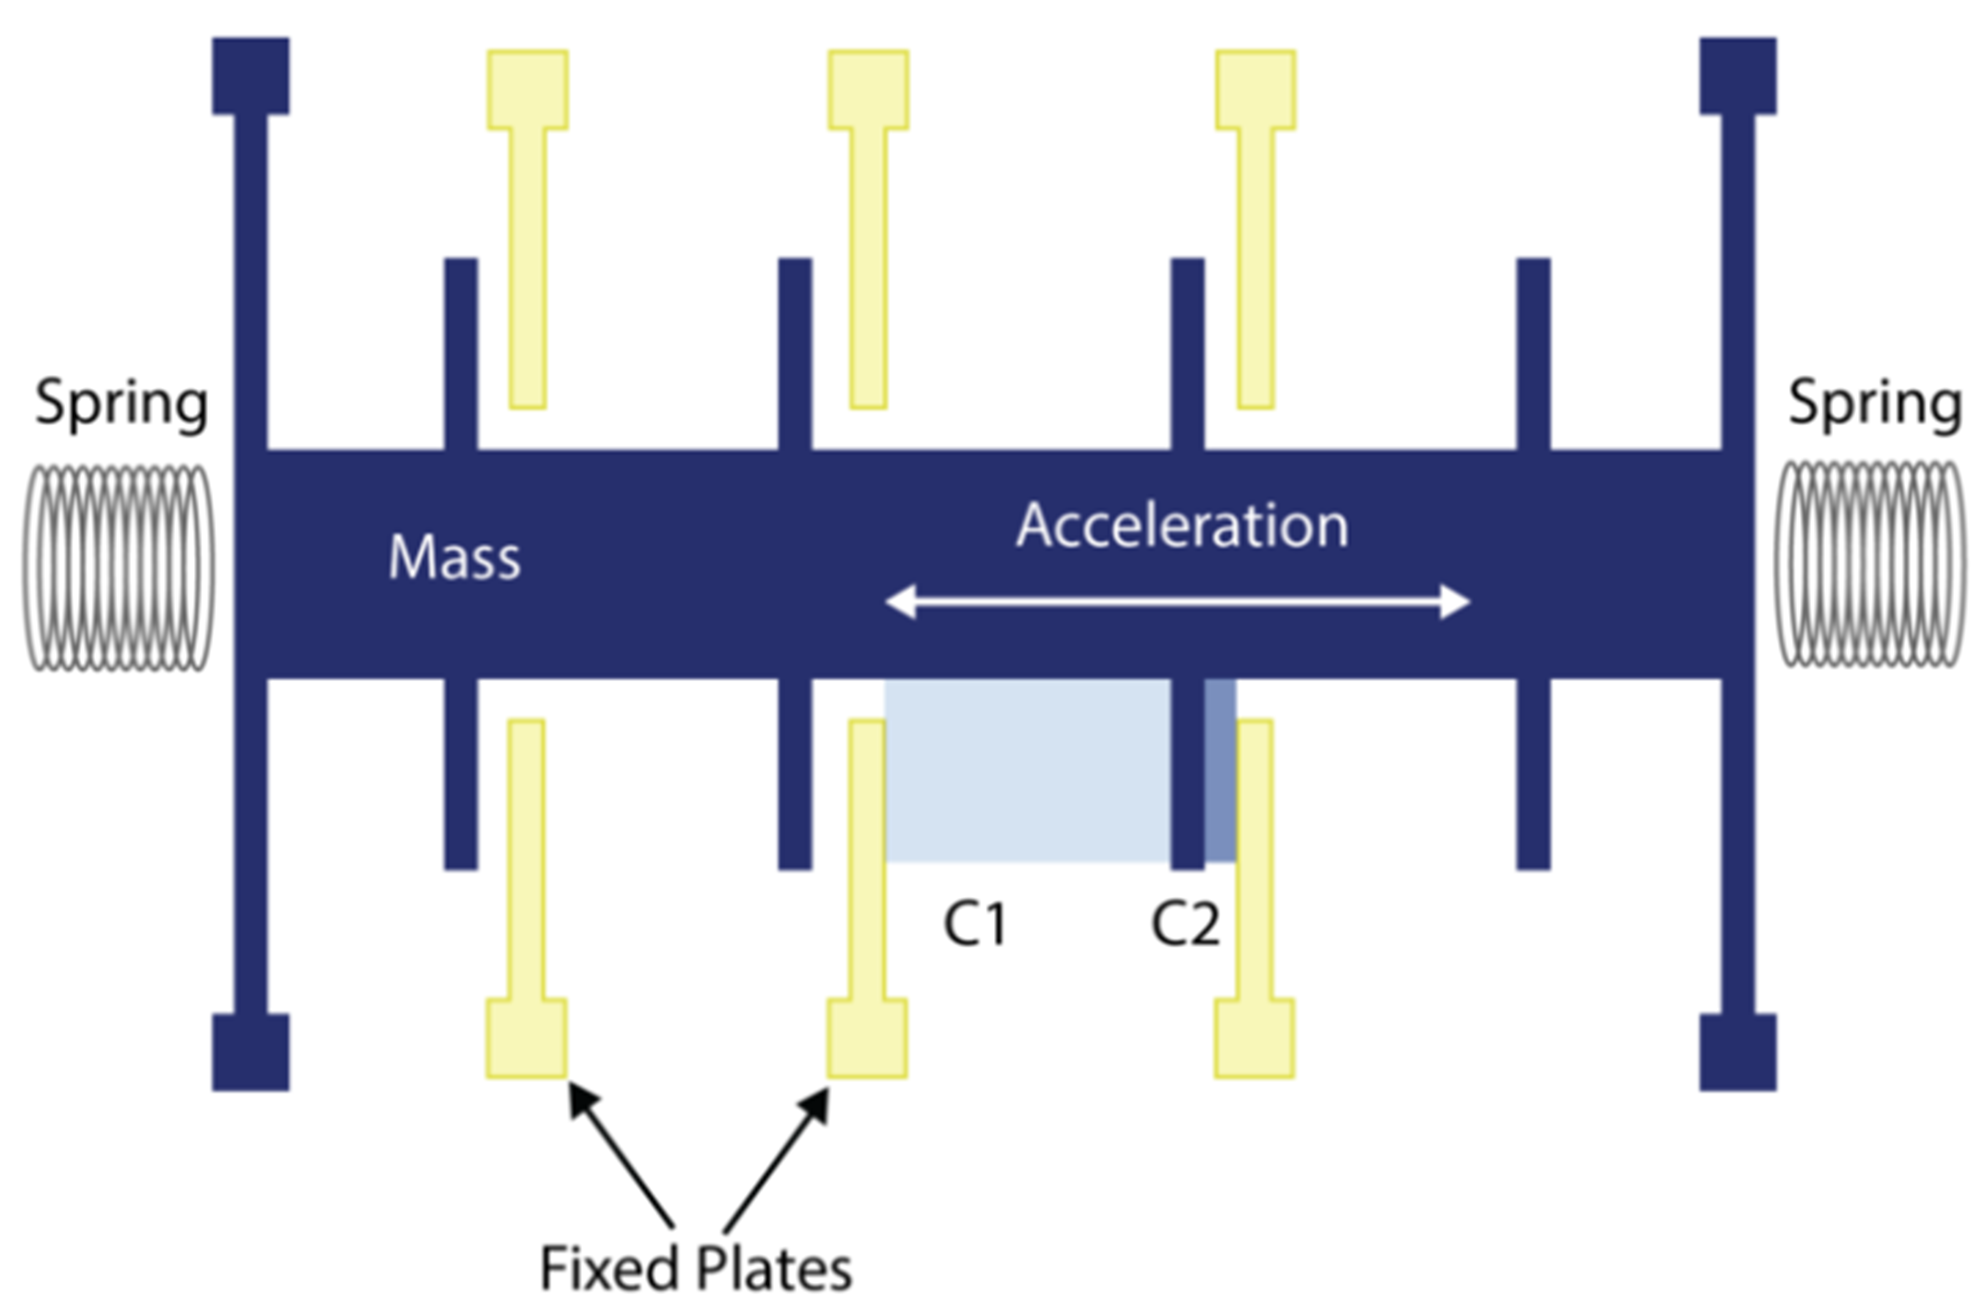
\includegraphics[width=0.5\columnwidth]{figures/mems-aks}
    \caption{MEMS-akselerometer. \parencite{LevelDevelopments2020}}
    \label{fig:mems-aks}
\end{figure}

\subsubsection{Piezoelektrisk akselerometer}
Den piezoelekstriske effekten kan også brukes til å beregne akselerasjon. 
Effekten går ut på at enkelte krystaller skaper en spenning ved deformering. \parencite{Gron2021piezo}
Ved å koble til elektroder på hver side av et krystall kan kraften av en masse som presser mot 
krystallen beregnes ut ifra spenningen som oppstår over krystallen. Ut ifra kraften og massens 
vekt kan akselerasjonen beregnes. Prinsippet for dette akselerometer er beskrevet ifigur \ref{fig:piezo-aks}. 
Basen vil være koblet statisk uelastisk til en gjenstand. Og når denne gjenstanden beveger seg i retningen som 
pilen viser vil en kunne beregne akselerasjonen ved hjelp av elektrodene på hver side av krystallen. 

\begin{figure}[htp]
\centering
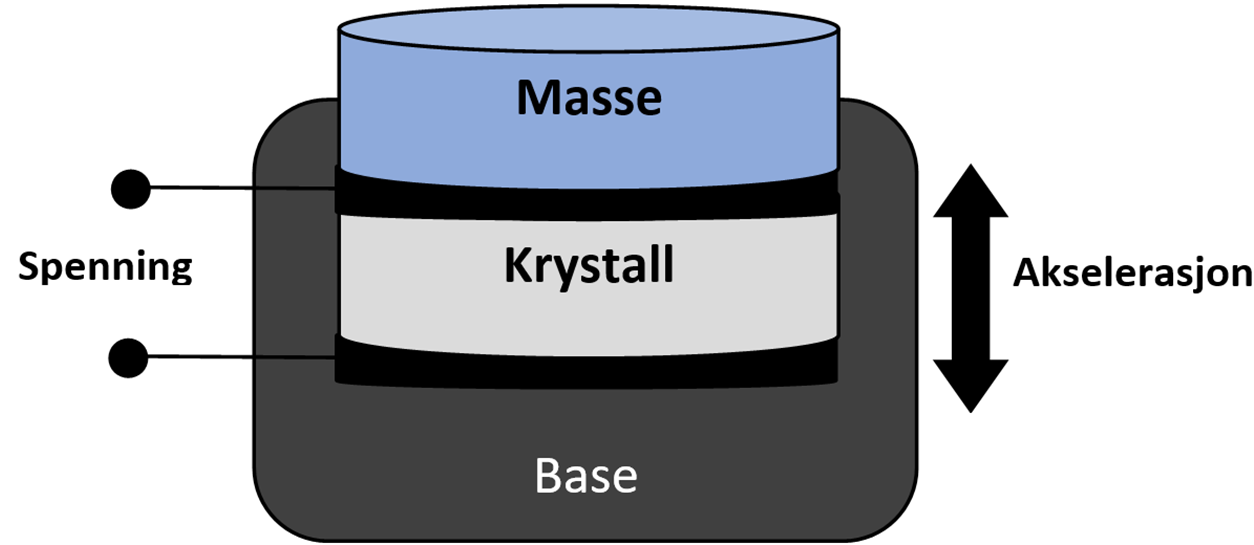
\includegraphics[width=0.5\columnwidth]{figures/piezo-aks}
\caption{Piezoelektrisk akselerometer.}
\label{fig:piezo-aks}
\end{figure}